% Created by tikzDevice version 0.10.1 on 2018-01-31 10:27:57
% !TEX encoding = UTF-8 Unicode
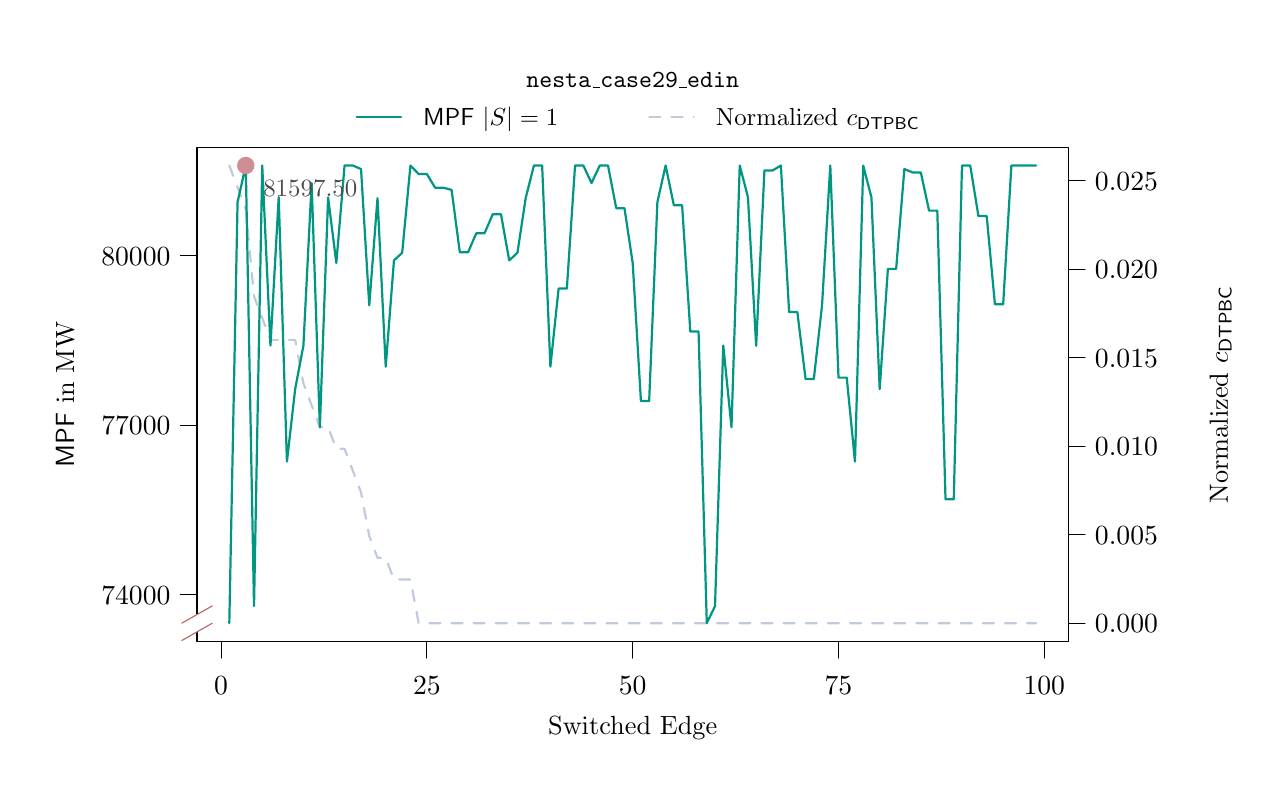
\begin{tikzpicture}[x=1pt,y=1pt]
\definecolor{fillColor}{RGB}{255,255,255}
\path[use as bounding box,fill=fillColor,fill opacity=0.00] (0,0) rectangle (440.85,271.01);
\begin{scope}
\path[clip] (  0.00,  0.00) rectangle (440.85,271.01);
\definecolor{drawColor}{RGB}{193,202,220}

\path[draw=drawColor,line width= 0.8pt,dash pattern=on 4pt off 4pt ,line join=round,line cap=round] ( 72.86,221.20) --
	( 75.84,213.32) --
	( 78.81,205.45) --
	( 81.79,173.95) --
	( 84.76,166.07) --
	( 87.73,158.19) --
	( 90.71,158.19) --
	( 93.68,158.19) --
	( 96.66,158.19) --
	( 99.63,142.44) --
	(102.61,134.57) --
	(105.58,126.69) --
	(108.56,126.69) --
	(111.53,118.82) --
	(114.51,118.82) --
	(117.48,110.94) --
	(120.46,103.07) --
	(123.43, 87.32) --
	(126.41, 79.44) --
	(129.38, 79.44) --
	(132.36, 71.57) --
	(135.33, 71.57) --
	(138.31, 71.57) --
	(141.28, 55.82) --
	(144.25, 55.82) --
	(147.23, 55.82) --
	(150.20, 55.82) --
	(153.18, 55.82) --
	(156.15, 55.82) --
	(159.13, 55.82) --
	(162.10, 55.82) --
	(165.08, 55.82) --
	(168.05, 55.82) --
	(171.03, 55.82) --
	(174.00, 55.82) --
	(176.98, 55.82) --
	(179.95, 55.82) --
	(182.93, 55.82) --
	(185.90, 55.82) --
	(188.88, 55.82) --
	(191.85, 55.82) --
	(194.83, 55.82) --
	(197.80, 55.82) --
	(200.78, 55.82) --
	(203.75, 55.82) --
	(206.72, 55.82) --
	(209.70, 55.82) --
	(212.67, 55.82) --
	(215.65, 55.82) --
	(218.62, 55.82) --
	(221.60, 55.82) --
	(224.57, 55.82) --
	(227.55, 55.82) --
	(230.52, 55.82) --
	(233.50, 55.82) --
	(236.47, 55.82) --
	(239.45, 55.82) --
	(242.42, 55.82) --
	(245.40, 55.82) --
	(248.37, 55.82) --
	(251.35, 55.82) --
	(254.32, 55.82) --
	(257.30, 55.82) --
	(260.27, 55.82) --
	(263.24, 55.82) --
	(266.22, 55.82) --
	(269.19, 55.82) --
	(272.17, 55.82) --
	(275.14, 55.82) --
	(278.12, 55.82) --
	(281.09, 55.82) --
	(284.07, 55.82) --
	(287.04, 55.82) --
	(290.02, 55.82) --
	(292.99, 55.82) --
	(295.97, 55.82) --
	(298.94, 55.82) --
	(301.92, 55.82) --
	(304.89, 55.82) --
	(307.87, 55.82) --
	(310.84, 55.82) --
	(313.82, 55.82) --
	(316.79, 55.82) --
	(319.76, 55.82) --
	(322.74, 55.82) --
	(325.71, 55.82) --
	(328.69, 55.82) --
	(331.66, 55.82) --
	(334.64, 55.82) --
	(337.61, 55.82) --
	(340.59, 55.82) --
	(343.56, 55.82) --
	(346.54, 55.82) --
	(349.51, 55.82) --
	(352.49, 55.82) --
	(355.46, 55.82) --
	(358.44, 55.82) --
	(361.41, 55.82) --
	(364.39, 55.82);
\end{scope}
\begin{scope}
\path[clip] (  0.00,  0.00) rectangle (440.85,271.01);
\definecolor{drawColor}{RGB}{0,0,0}

\path[draw=drawColor,line width= 0.4pt,line join=round,line cap=round] ( 61.20, 49.20) --
	(376.05, 49.20) --
	(376.05,227.81) --
	( 61.20,227.81) --
	( 61.20, 49.20);
\end{scope}
\begin{scope}
\path[clip] (  0.00,  0.00) rectangle (440.85,271.01);
\definecolor{drawColor}{RGB}{0,0,0}

\path[draw=drawColor,line width= 0.4pt,line join=round,line cap=round] (376.05, 55.82) -- (376.05,215.68);

\path[draw=drawColor,line width= 0.4pt,line join=round,line cap=round] (376.05, 55.82) -- (382.05, 55.82);

\path[draw=drawColor,line width= 0.4pt,line join=round,line cap=round] (376.05, 87.79) -- (382.05, 87.79);

\path[draw=drawColor,line width= 0.4pt,line join=round,line cap=round] (376.05,119.76) -- (382.05,119.76);

\path[draw=drawColor,line width= 0.4pt,line join=round,line cap=round] (376.05,151.74) -- (382.05,151.74);

\path[draw=drawColor,line width= 0.4pt,line join=round,line cap=round] (376.05,183.71) -- (382.05,183.71);

\path[draw=drawColor,line width= 0.4pt,line join=round,line cap=round] (376.05,215.68) -- (382.05,215.68);

\node[text=drawColor,anchor=base west,inner sep=0pt, outer sep=0pt, scale=  1.00] at (385.65, 52.37) {0.000};

\node[text=drawColor,anchor=base west,inner sep=0pt, outer sep=0pt, scale=  1.00] at (385.65, 84.35) {0.005};

\node[text=drawColor,anchor=base west,inner sep=0pt, outer sep=0pt, scale=  1.00] at (385.65,116.32) {0.010};

\node[text=drawColor,anchor=base west,inner sep=0pt, outer sep=0pt, scale=  1.00] at (385.65,148.29) {0.015};

\node[text=drawColor,anchor=base west,inner sep=0pt, outer sep=0pt, scale=  1.00] at (385.65,180.27) {0.020};

\node[text=drawColor,anchor=base west,inner sep=0pt, outer sep=0pt, scale=  1.00] at (385.65,212.24) {0.025};
\end{scope}
\begin{scope}
\path[clip] (  0.00,  0.00) rectangle (440.85,271.01);
\definecolor{drawColor}{RGB}{0,150,130}

\path[draw=drawColor,line width= 0.8pt,line join=round,line cap=round] (118.89,238.60) -- (134.91,238.60);
\definecolor{drawColor}{RGB}{193,202,220}

\path[draw=drawColor,line width= 0.8pt,dash pattern=on 4pt off 4pt ,line join=round,line cap=round] (224.63,238.60) -- (240.65,238.60);
\definecolor{drawColor}{RGB}{0,0,0}

\node[text=drawColor,anchor=base,inner sep=0pt, outer sep=0pt, scale=  0.89] at (218.62,249.28) {\texttt{nesta\_case29\_edin}};

\node[text=drawColor,anchor=base west,inner sep=0pt, outer sep=0pt, scale=  0.89] at (142.92,235.54) {$\mathsf{MPF}~|S|=1$};

\node[text=drawColor,anchor=base west,inner sep=0pt, outer sep=0pt, scale=  0.89] at (248.66,235.54) {Normalized~$c_\mathsf{DTPBC}$};
\end{scope}
\begin{scope}
\path[clip] (  0.00,  0.00) rectangle (440.85,271.01);
\definecolor{drawColor}{RGB}{0,0,0}

\path[draw=drawColor,line width= 0.4pt,line join=round,line cap=round] ( 61.20, 66.16) -- ( 61.20,188.60);

\path[draw=drawColor,line width= 0.4pt,line join=round,line cap=round] ( 61.20, 66.16) -- ( 55.20, 66.16);

\path[draw=drawColor,line width= 0.4pt,line join=round,line cap=round] ( 61.20,127.38) -- ( 55.20,127.38);

\path[draw=drawColor,line width= 0.4pt,line join=round,line cap=round] ( 61.20,188.60) -- ( 55.20,188.60);

\node[text=drawColor,anchor=base east,inner sep=0pt, outer sep=0pt, scale=  1.00] at ( 51.60, 62.72) {74000};

\node[text=drawColor,anchor=base east,inner sep=0pt, outer sep=0pt, scale=  1.00] at ( 51.60,123.94) {77000};

\node[text=drawColor,anchor=base east,inner sep=0pt, outer sep=0pt, scale=  1.00] at ( 51.60,185.16) {80000};
\end{scope}
\begin{scope}
\path[clip] (  0.00,  0.00) rectangle (440.85,271.01);
\definecolor{drawColor}{RGB}{255,255,255}
\definecolor{fillColor}{RGB}{255,255,255}

\path[draw=drawColor,line width= 0.4pt,line join=round,line cap=round,fill=fillColor] ( 55.69, 52.69) rectangle ( 66.71, 58.94);
\definecolor{drawColor}{RGB}{188,97,104}

\path[draw=drawColor,line width= 0.4pt,line join=round,line cap=round] ( 55.69, 49.56) -- ( 66.71, 55.82);

\path[draw=drawColor,line width= 0.4pt,line join=round,line cap=round] ( 55.69, 55.82) -- ( 66.71, 62.07);
\end{scope}
\begin{scope}
\path[clip] ( 61.20, 49.20) rectangle (376.05,227.81);
\definecolor{drawColor}{RGB}{0,150,130}

\path[draw=drawColor,line width= 0.8pt,line join=round,line cap=round] ( 72.86, 55.82) --
	( 75.84,208.00) --
	( 78.81,221.20) --
	( 81.79, 61.99) --
	( 84.76,221.20) --
	( 87.73,156.14) --
	( 90.71,209.78) --
	( 93.68,114.20) --
	( 96.66,140.42) --
	( 99.63,156.06) --
	(102.61,214.86) --
	(105.58,126.59) --
	(108.56,209.67) --
	(111.53,186.00) --
	(114.51,221.20) --
	(117.48,221.20) --
	(120.46,219.91) --
	(123.43,170.67) --
	(126.41,209.40) --
	(129.38,148.52) --
	(132.36,186.92) --
	(135.33,189.67) --
	(138.31,221.20) --
	(141.28,218.12) --
	(144.25,218.12) --
	(147.23,213.17) --
	(150.20,213.17) --
	(153.18,212.40) --
	(156.15,189.86) --
	(159.13,189.86) --
	(162.10,196.71) --
	(165.08,196.71) --
	(168.05,203.58) --
	(171.03,203.58) --
	(174.00,186.92) --
	(176.98,189.67) --
	(179.95,209.40) --
	(182.93,221.20) --
	(185.90,221.20) --
	(188.88,148.52) --
	(191.85,176.73) --
	(194.83,176.73) --
	(197.80,221.20) --
	(200.78,221.20) --
	(203.75,214.86) --
	(206.72,221.20) --
	(209.70,221.20) --
	(212.67,205.79) --
	(215.65,205.79) --
	(218.62,186.00) --
	(221.60,136.07) --
	(224.57,136.07) --
	(227.55,208.00) --
	(230.52,221.20) --
	(233.50,206.82) --
	(236.47,206.82) --
	(239.45,161.19) --
	(242.42,161.19) --
	(245.40, 55.82) --
	(248.37, 61.99) --
	(251.35,156.14) --
	(254.32,126.59) --
	(257.30,221.20) --
	(260.27,209.78) --
	(263.24,156.06) --
	(266.22,219.42) --
	(269.19,219.42) --
	(272.17,221.20) --
	(275.14,168.24) --
	(278.12,168.24) --
	(281.09,144.02) --
	(284.07,144.02) --
	(287.04,170.67) --
	(290.02,221.20) --
	(292.99,144.55) --
	(295.97,144.55) --
	(298.94,114.20) --
	(301.92,221.20) --
	(304.89,209.67) --
	(307.87,140.42) --
	(310.84,183.85) --
	(313.82,183.85) --
	(316.79,219.91) --
	(319.76,218.70) --
	(322.74,218.70) --
	(325.71,204.90) --
	(328.69,204.90) --
	(331.66,100.57) --
	(334.64,100.57) --
	(337.61,221.20) --
	(340.59,221.20) --
	(343.56,202.92) --
	(346.54,202.92) --
	(349.51,171.06) --
	(352.49,171.06) --
	(355.46,221.20) --
	(358.44,221.20) --
	(361.41,221.20) --
	(364.39,221.20);
\end{scope}
\begin{scope}
\path[clip] ( 61.20, 49.20) rectangle (376.05,227.81);
\definecolor{fillColor}{RGB}{207,142,147}

\path[fill=fillColor] ( 78.81,221.20) circle (  3.15);
\end{scope}
\begin{scope}
\path[clip] ( 61.20, 49.20) rectangle (376.05,227.81);
\definecolor{drawColor}{gray}{0.30}

\node[text=drawColor,anchor=base,inner sep=0pt, outer sep=0pt, scale=  0.90] at (102.13,210.04) {81597.50};
\end{scope}
\begin{scope}
\path[clip] (  0.00,  0.00) rectangle (440.85,271.01);
\definecolor{drawColor}{RGB}{0,0,0}

\path[draw=drawColor,line width= 0.4pt,line join=round,line cap=round] ( 69.89, 49.20) -- (367.36, 49.20);

\path[draw=drawColor,line width= 0.4pt,line join=round,line cap=round] ( 69.89, 49.20) -- ( 69.89, 43.20);

\path[draw=drawColor,line width= 0.4pt,line join=round,line cap=round] (144.25, 49.20) -- (144.25, 43.20);

\path[draw=drawColor,line width= 0.4pt,line join=round,line cap=round] (218.62, 49.20) -- (218.62, 43.20);

\path[draw=drawColor,line width= 0.4pt,line join=round,line cap=round] (292.99, 49.20) -- (292.99, 43.20);

\path[draw=drawColor,line width= 0.4pt,line join=round,line cap=round] (367.36, 49.20) -- (367.36, 43.20);

\node[text=drawColor,anchor=base,inner sep=0pt, outer sep=0pt, scale=  1.00] at ( 69.89, 30.00) {0};

\node[text=drawColor,anchor=base,inner sep=0pt, outer sep=0pt, scale=  1.00] at (144.25, 30.00) {25};

\node[text=drawColor,anchor=base,inner sep=0pt, outer sep=0pt, scale=  1.00] at (218.62, 30.00) {50};

\node[text=drawColor,anchor=base,inner sep=0pt, outer sep=0pt, scale=  1.00] at (292.99, 30.00) {75};

\node[text=drawColor,anchor=base,inner sep=0pt, outer sep=0pt, scale=  1.00] at (367.36, 30.00) {100};

\node[text=drawColor,anchor=base,inner sep=0pt, outer sep=0pt, scale=  0.95] at (218.62, 15.60) {Switched Edge};

\node[text=drawColor,rotate= 90.00,anchor=base,inner sep=0pt, outer sep=0pt, scale=  0.95] at ( 16.80,138.51) {$\mathsf{MPF}$ in~$\mathrm{MW}$};

\node[text=drawColor,rotate= 90.00,anchor=base,inner sep=0pt, outer sep=0pt, scale=  0.95] at (433.65,138.51) {Normalized~$c_\mathsf{DTPBC}$};
\end{scope}
\end{tikzpicture}
